% Created by tikzDevice version 0.10.1 on 2018-03-04 20:38:39
% !TEX encoding = UTF-8 Unicode
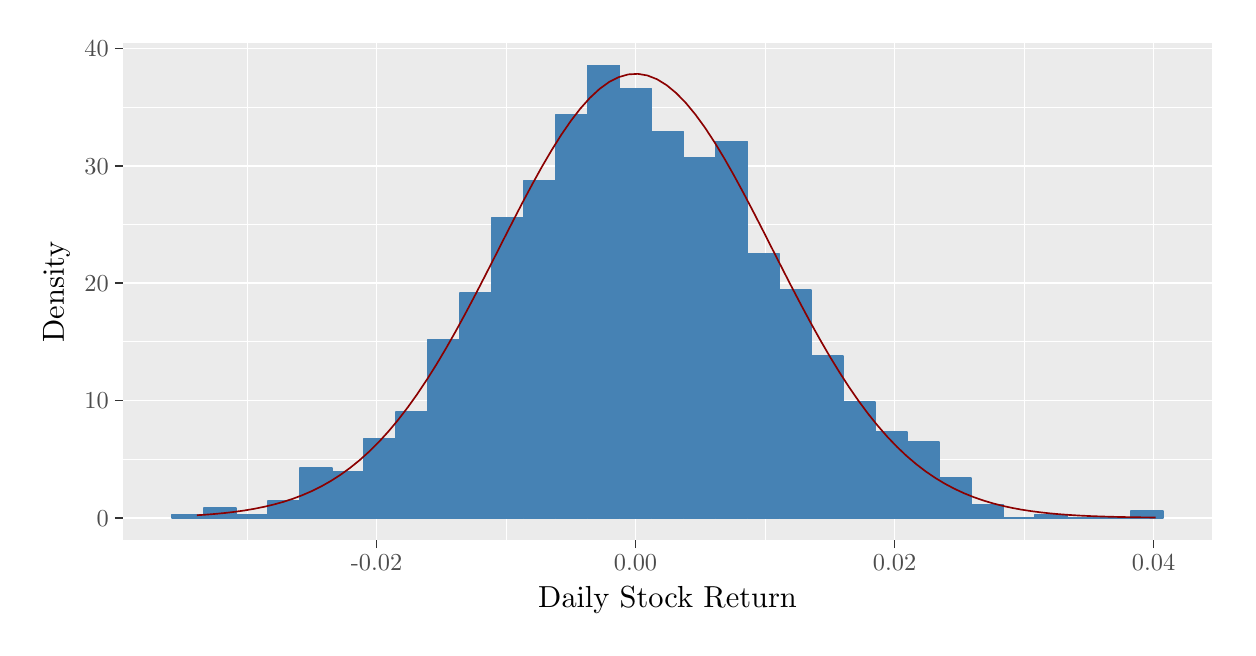
\begin{tikzpicture}[x=1pt,y=1pt]
\definecolor{fillColor}{RGB}{255,255,255}
\path[use as bounding box,fill=fillColor,fill opacity=0.00] (0,0) rectangle (433.62,216.81);
\begin{scope}
\path[clip] (  0.00,  0.00) rectangle (433.62,216.81);
\definecolor{drawColor}{RGB}{255,255,255}
\definecolor{fillColor}{RGB}{255,255,255}

\path[draw=drawColor,line width= 0.6pt,line join=round,line cap=round,fill=fillColor] (  0.00,  0.00) rectangle (433.62,216.81);
\end{scope}
\begin{scope}
\path[clip] ( 34.27, 31.53) rectangle (428.12,211.31);
\definecolor{fillColor}{gray}{0.92}

\path[fill=fillColor] ( 34.27, 31.53) rectangle (428.12,211.31);
\definecolor{drawColor}{RGB}{255,255,255}

\path[draw=drawColor,line width= 0.3pt,line join=round] ( 34.27, 60.90) --
	(428.12, 60.90);

\path[draw=drawColor,line width= 0.3pt,line join=round] ( 34.27,103.29) --
	(428.12,103.29);

\path[draw=drawColor,line width= 0.3pt,line join=round] ( 34.27,145.69) --
	(428.12,145.69);

\path[draw=drawColor,line width= 0.3pt,line join=round] ( 34.27,188.08) --
	(428.12,188.08);

\path[draw=drawColor,line width= 0.3pt,line join=round] ( 79.24, 31.53) --
	( 79.24,211.31);

\path[draw=drawColor,line width= 0.3pt,line join=round] (172.84, 31.53) --
	(172.84,211.31);

\path[draw=drawColor,line width= 0.3pt,line join=round] (266.45, 31.53) --
	(266.45,211.31);

\path[draw=drawColor,line width= 0.3pt,line join=round] (360.05, 31.53) --
	(360.05,211.31);

\path[draw=drawColor,line width= 0.6pt,line join=round] ( 34.27, 39.70) --
	(428.12, 39.70);

\path[draw=drawColor,line width= 0.6pt,line join=round] ( 34.27, 82.10) --
	(428.12, 82.10);

\path[draw=drawColor,line width= 0.6pt,line join=round] ( 34.27,124.49) --
	(428.12,124.49);

\path[draw=drawColor,line width= 0.6pt,line join=round] ( 34.27,166.88) --
	(428.12,166.88);

\path[draw=drawColor,line width= 0.6pt,line join=round] ( 34.27,209.28) --
	(428.12,209.28);

\path[draw=drawColor,line width= 0.6pt,line join=round] (126.04, 31.53) --
	(126.04,211.31);

\path[draw=drawColor,line width= 0.6pt,line join=round] (219.64, 31.53) --
	(219.64,211.31);

\path[draw=drawColor,line width= 0.6pt,line join=round] (313.25, 31.53) --
	(313.25,211.31);

\path[draw=drawColor,line width= 0.6pt,line join=round] (406.85, 31.53) --
	(406.85,211.31);
\definecolor{drawColor}{RGB}{70,130,180}
\definecolor{fillColor}{RGB}{70,130,180}

\path[draw=drawColor,line width= 0.6pt,line join=round,fill=fillColor] ( 52.17, 39.70) rectangle ( 63.72, 40.90);

\path[draw=drawColor,line width= 0.6pt,line join=round,fill=fillColor] ( 63.72, 39.70) rectangle ( 75.27, 43.28);

\path[draw=drawColor,line width= 0.6pt,line join=round,fill=fillColor] ( 75.27, 39.70) rectangle ( 86.82, 40.90);

\path[draw=drawColor,line width= 0.6pt,line join=round,fill=fillColor] ( 86.82, 39.70) rectangle ( 98.37, 45.67);

\path[draw=drawColor,line width= 0.6pt,line join=round,fill=fillColor] ( 98.37, 39.70) rectangle (109.92, 57.60);

\path[draw=drawColor,line width= 0.6pt,line join=round,fill=fillColor] (109.92, 39.70) rectangle (121.47, 56.40);

\path[draw=drawColor,line width= 0.6pt,line join=round,fill=fillColor] (121.47, 39.70) rectangle (133.02, 68.33);

\path[draw=drawColor,line width= 0.6pt,line join=round,fill=fillColor] (133.02, 39.70) rectangle (144.57, 77.88);

\path[draw=drawColor,line width= 0.6pt,line join=round,fill=fillColor] (144.57, 39.70) rectangle (156.12,104.12);

\path[draw=drawColor,line width= 0.6pt,line join=round,fill=fillColor] (156.12, 39.70) rectangle (167.67,120.82);

\path[draw=drawColor,line width= 0.6pt,line join=round,fill=fillColor] (167.67, 39.70) rectangle (179.22,148.26);

\path[draw=drawColor,line width= 0.6pt,line join=round,fill=fillColor] (179.22, 39.70) rectangle (190.77,161.38);

\path[draw=drawColor,line width= 0.6pt,line join=round,fill=fillColor] (190.77, 39.70) rectangle (202.32,185.24);

\path[draw=drawColor,line width= 0.6pt,line join=round,fill=fillColor] (202.32, 39.70) rectangle (213.87,203.14);

\path[draw=drawColor,line width= 0.6pt,line join=round,fill=fillColor] (213.87, 39.70) rectangle (225.42,194.79);

\path[draw=drawColor,line width= 0.6pt,line join=round,fill=fillColor] (225.42, 39.70) rectangle (236.97,179.28);

\path[draw=drawColor,line width= 0.6pt,line join=round,fill=fillColor] (236.97, 39.70) rectangle (248.52,169.74);

\path[draw=drawColor,line width= 0.6pt,line join=round,fill=fillColor] (248.52, 39.70) rectangle (260.07,175.70);

\path[draw=drawColor,line width= 0.6pt,line join=round,fill=fillColor] (260.07, 39.70) rectangle (271.62,135.14);

\path[draw=drawColor,line width= 0.6pt,line join=round,fill=fillColor] (271.62, 39.70) rectangle (283.17,122.02);

\path[draw=drawColor,line width= 0.6pt,line join=round,fill=fillColor] (283.17, 39.70) rectangle (294.72, 98.16);

\path[draw=drawColor,line width= 0.6pt,line join=round,fill=fillColor] (294.72, 39.70) rectangle (306.27, 81.46);

\path[draw=drawColor,line width= 0.6pt,line join=round,fill=fillColor] (306.27, 39.70) rectangle (317.82, 70.72);

\path[draw=drawColor,line width= 0.6pt,line join=round,fill=fillColor] (317.82, 39.70) rectangle (329.37, 67.14);

\path[draw=drawColor,line width= 0.6pt,line join=round,fill=fillColor] (329.37, 39.70) rectangle (340.92, 54.02);

\path[draw=drawColor,line width= 0.6pt,line join=round,fill=fillColor] (340.92, 39.70) rectangle (352.47, 44.47);

\path[draw=drawColor,line width= 0.6pt,line join=round,fill=fillColor] (352.47, 39.70) rectangle (364.02, 39.70);

\path[draw=drawColor,line width= 0.6pt,line join=round,fill=fillColor] (364.02, 39.70) rectangle (375.57, 40.90);

\path[draw=drawColor,line width= 0.6pt,line join=round,fill=fillColor] (375.57, 39.70) rectangle (387.12, 39.70);

\path[draw=drawColor,line width= 0.6pt,line join=round,fill=fillColor] (387.12, 39.70) rectangle (398.67, 39.70);

\path[draw=drawColor,line width= 0.6pt,line join=round,fill=fillColor] (398.67, 39.70) rectangle (410.22, 42.09);
\definecolor{drawColor}{RGB}{139,0,0}

\path[draw=drawColor,line width= 0.6pt,line join=round] ( 61.12, 40.62) --
	( 64.59, 40.85) --
	( 68.05, 41.13) --
	( 71.52, 41.47) --
	( 74.98, 41.88) --
	( 78.45, 42.37) --
	( 81.91, 42.96) --
	( 85.38, 43.66) --
	( 88.84, 44.48) --
	( 92.31, 45.44) --
	( 95.77, 46.56) --
	( 99.24, 47.87) --
	(102.70, 49.37) --
	(106.17, 51.09) --
	(109.63, 53.06) --
	(113.10, 55.28) --
	(116.56, 57.79) --
	(120.03, 60.59) --
	(123.49, 63.72) --
	(126.96, 67.17) --
	(130.42, 70.97) --
	(133.89, 75.12) --
	(137.35, 79.62) --
	(140.82, 84.47) --
	(144.28, 89.66) --
	(147.75, 95.18) --
	(151.21,101.01) --
	(154.68,107.12) --
	(158.14,113.47) --
	(161.61,120.02) --
	(165.07,126.73) --
	(168.54,133.52) --
	(172.00,140.36) --
	(175.47,147.15) --
	(178.93,153.85) --
	(182.40,160.36) --
	(185.86,166.62) --
	(189.33,172.54) --
	(192.79,178.06) --
	(196.26,183.10) --
	(199.72,187.59) --
	(203.19,191.47) --
	(206.65,194.68) --
	(210.12,197.19) --
	(213.58,198.94) --
	(217.05,199.93) --
	(220.51,200.12) --
	(223.98,199.53) --
	(227.44,198.16) --
	(230.91,196.02) --
	(234.37,193.16) --
	(237.84,189.60) --
	(241.30,185.41) --
	(244.77,180.64) --
	(248.23,175.35) --
	(251.70,169.62) --
	(255.16,163.52) --
	(258.63,157.12) --
	(262.09,150.51) --
	(265.56,143.76) --
	(269.02,136.93) --
	(272.49,130.11) --
	(275.95,123.35) --
	(279.42,116.72) --
	(282.88,110.26) --
	(286.35,104.03) --
	(289.81, 98.05) --
	(293.28, 92.38) --
	(296.74, 87.02) --
	(300.21, 81.99) --
	(303.67, 77.32) --
	(307.14, 73.00) --
	(310.60, 69.02) --
	(314.07, 65.40) --
	(317.53, 62.11) --
	(321.00, 59.15) --
	(324.46, 56.49) --
	(327.93, 54.13) --
	(331.39, 52.04) --
	(334.86, 50.20) --
	(338.32, 48.59) --
	(341.79, 47.19) --
	(345.25, 45.98) --
	(348.72, 44.94) --
	(352.18, 44.05) --
	(355.65, 43.29) --
	(359.11, 42.65) --
	(362.58, 42.12) --
	(366.04, 41.67) --
	(369.51, 41.29) --
	(372.97, 40.98) --
	(376.44, 40.73) --
	(379.90, 40.52) --
	(383.37, 40.35) --
	(386.83, 40.22) --
	(390.30, 40.11) --
	(393.76, 40.02) --
	(397.23, 39.95) --
	(400.69, 39.89) --
	(404.16, 39.85) --
	(407.62, 39.82);
\end{scope}
\begin{scope}
\path[clip] (  0.00,  0.00) rectangle (433.62,216.81);
\definecolor{drawColor}{gray}{0.30}

\node[text=drawColor,anchor=base east,inner sep=0pt, outer sep=0pt, scale=  0.88] at ( 29.32, 36.67) {0};

\node[text=drawColor,anchor=base east,inner sep=0pt, outer sep=0pt, scale=  0.88] at ( 29.32, 79.07) {10};

\node[text=drawColor,anchor=base east,inner sep=0pt, outer sep=0pt, scale=  0.88] at ( 29.32,121.46) {20};

\node[text=drawColor,anchor=base east,inner sep=0pt, outer sep=0pt, scale=  0.88] at ( 29.32,163.85) {30};

\node[text=drawColor,anchor=base east,inner sep=0pt, outer sep=0pt, scale=  0.88] at ( 29.32,206.25) {40};
\end{scope}
\begin{scope}
\path[clip] (  0.00,  0.00) rectangle (433.62,216.81);
\definecolor{drawColor}{gray}{0.20}

\path[draw=drawColor,line width= 0.6pt,line join=round] ( 31.52, 39.70) --
	( 34.27, 39.70);

\path[draw=drawColor,line width= 0.6pt,line join=round] ( 31.52, 82.10) --
	( 34.27, 82.10);

\path[draw=drawColor,line width= 0.6pt,line join=round] ( 31.52,124.49) --
	( 34.27,124.49);

\path[draw=drawColor,line width= 0.6pt,line join=round] ( 31.52,166.88) --
	( 34.27,166.88);

\path[draw=drawColor,line width= 0.6pt,line join=round] ( 31.52,209.28) --
	( 34.27,209.28);
\end{scope}
\begin{scope}
\path[clip] (  0.00,  0.00) rectangle (433.62,216.81);
\definecolor{drawColor}{gray}{0.20}

\path[draw=drawColor,line width= 0.6pt,line join=round] (126.04, 28.78) --
	(126.04, 31.53);

\path[draw=drawColor,line width= 0.6pt,line join=round] (219.64, 28.78) --
	(219.64, 31.53);

\path[draw=drawColor,line width= 0.6pt,line join=round] (313.25, 28.78) --
	(313.25, 31.53);

\path[draw=drawColor,line width= 0.6pt,line join=round] (406.85, 28.78) --
	(406.85, 31.53);
\end{scope}
\begin{scope}
\path[clip] (  0.00,  0.00) rectangle (433.62,216.81);
\definecolor{drawColor}{gray}{0.30}

\node[text=drawColor,anchor=base,inner sep=0pt, outer sep=0pt, scale=  0.88] at (126.04, 20.52) {-0.02};

\node[text=drawColor,anchor=base,inner sep=0pt, outer sep=0pt, scale=  0.88] at (219.64, 20.52) {0.00};

\node[text=drawColor,anchor=base,inner sep=0pt, outer sep=0pt, scale=  0.88] at (313.25, 20.52) {0.02};

\node[text=drawColor,anchor=base,inner sep=0pt, outer sep=0pt, scale=  0.88] at (406.85, 20.52) {0.04};
\end{scope}
\begin{scope}
\path[clip] (  0.00,  0.00) rectangle (433.62,216.81);
\definecolor{drawColor}{RGB}{0,0,0}

\node[text=drawColor,anchor=base,inner sep=0pt, outer sep=0pt, scale=  1.10] at (231.19,  7.44) {Daily Stock Return};
\end{scope}
\begin{scope}
\path[clip] (  0.00,  0.00) rectangle (433.62,216.81);
\definecolor{drawColor}{RGB}{0,0,0}

\node[text=drawColor,rotate= 90.00,anchor=base,inner sep=0pt, outer sep=0pt, scale=  1.10] at ( 13.08,121.42) {Density};
\end{scope}
\end{tikzpicture}
